% !TEX root = main.tex

\documentclass{Interspeech}

\usepackage{todonotes}
\usepackage{hyperref}
\hypersetup{
    colorlinks=true,
    linkcolor=black,
    filecolor=magenta,      
    urlcolor=red,
    pdftitle={Defence Against the Deepfake Arts},
    pdfpagemode=FullScreen,
}

% 2023-10-21 modified by Simon King (Simon.King@ed.ac.uk)  
% 2024-01 modified by TPC Chairs of Interspeech 2024  
% 2024-10 modified by Antoine Serrurier for Interspeech 2025
% 2024-12 modified by TPC Chairs of Interspeech 2025
% 2025-02 modified by Team DADA

% ************************************* *
% *    DOUBLE-BLIND REVIEW SETTINGS    *
% **************************************
% Comment out \interspeechcameraready when submitting the 
% paper for review.
% If your paper is accepted, uncomment this to produce the
%  'camera ready' version to submit for publication.

% \interspeechcameraready


% **************************************
% *                                    *
% *      STOP !   DO NOT DELETE !      *
% *          READ THIS FIRST           *
% *                                    *
% * This template also includes        *
% * important INSTRUCTIONS that you    *
% * must follow when preparing your    *
% * paper. Read it BEFORE replacing    *
% * the content with your own work.    *
% **************************************

% title here must exactly match the title entered into the paper submission system
\title{Defence Against the Deepfake Arts : Improving Audio Deepfake Detection With Context Awareness}

% the order of authors here must exactly match the order entered into the paper submission system
% note that the COMPLETE list of authors MUST be entered into the paper submission system at the outset, including when submitting your manuscript for double-blind review
\author[affiliation={1, 2*}]{Nicoline}{Nymand-Andersen}
\author[affiliation={1*}]{Ivanina}{Ivanova}
\author[affiliation={1*}]{Abhay}{Dayal Mathur}
\author[affiliation={1}]{Nils}{Holzenberger}


%The maximum number of authors in the author list is 20. If the number of contributing authors is more than this, they should be listed in a footnote or the acknowledgement section.

% if you have too many addresses to fit within the available space, try removing the "\\" newlines
\affiliation{Telecom Paris}{Institut Polytechnique de Paris}{France}
\affiliation{Department of Computer Science}{Technische Universität München}{Germany}
% \affiliation{}{Just Institute}{And Country}
\email{nnymand-23@ip-paris.fr, ivanina.ivanova@ip-paris.fr, abhay.mathur@ip-paris.fr, nils.holzenberger@telecom-paris.fr}
\keywords{audio deepfake detection}

\newcommand{\blue}[1]{\textcolor{blue}{#1}}
\usepackage{comment}

\begin{document}

\maketitle

% the abstract here must exactly match the abstract entered into the paper submission system
\begin{abstract}

  % 1000 characters. ASCII characters only. No citations.
  \todo[inline]{Abhay : Exceeding 408 characters.}
  The increasing use of generative AI models to create realistic deepfakes poses significant challenges to information security, particularly in the realm of audio manipulation. This paper addresses the pressing need for improved detection of audio deepfakes by proposing a novel approach that incorporates context awareness. We begin by discussing the various types of audio deepfakes and their potential consequences, emphasising their ethical considerations and threats to privacy, security, and democratic processes. We review existing deepfake detection techniques and currently identified challenges in the field. We then present our method, which leverages textual context extracted from transcriptions as well as audio features extracted from deepfake detection models. We propose two fusion strategies, late fusion and mid fusion, to integrate these features and enhance detection accuracy. We conduct experiments using benchmark datasets and state-of-the-art deepfake detection models to evaluate the performance of our proposed approach. Our results demonstrate promising improvements in detecting audio deepfakes, highlighting the potential of context awareness in enhancing detection capabilities. Finally, we discuss the implications of our findings, including the privacy-security trade-off and limitations of our approach, and suggest directions for future research to address these challenges.
\end{abstract}

\section{Introduction}
\label{sec:introduction}

With the rapid advances of the digital landscape and new media technologies,
users become increasingly exposed to different types of manipulations.
Nowadays, everyone can create super realistic AI-generated content such as
images, audio, and even videos. The challenge of distinguishing between those
and the real ones becomes nearly impossible for the ordinary user. Audio
deepfakes or voice clones are like digital ventriloquists, using various deep
learning techniques to create voices that convincingly impersonate real
people~\cite{adversarial}. We can distinguish between a couple of different
types of deepfakes.~\cite{review_audio_deepfake_issues}. The first approach is
imitation-based (voice conversion), wherein the original audio signal is
modified to mimic another targeted voice. The manipulations can be of the
speech style, tone, and articulation. This technique is mainly used in show
business and, therefore, is applied by a third person or deep learning
software.

The second approach is synthetic-based, which produces artificially generated
speech by using text-to-speech techniques (TTS). This process involves three
stages: text analysis, acoustic, and vocoder. The text analysis step gathers
related audio files and the corresponding transcripts. Next, the acoustic
module extracts relevant features from the collected audio files to train the
new model. Techniques like Tacotron 2, Deep Voice 3~\cite{ping2018deep}, and
Flat Speech 2~\cite{ren2022fastspeech} are being used for this module. Finally,
the vocoder generates the final deepfake audio output by creating a speech
waveform based on the information extracted from the steps before.

The third technique is centred on replaying existing recordings of the target
speaker. Two techniques are notable here: cut-and-paste detection, where a
victim's recorded segment is played through a phone handset for capture, and
far-field detection, which involves crafting sentences for manipulation of a
text-dependent system.

There are other types of deepfakes, such as emotion fake. This technique alters
the emotions of a speaker's voice while preserving the original words and
speaker identity. For example, a happy statement can be transformed into a
sorrowful one, potentially twisting the meaning and intent of the
message~\cite{zhao2023emofake}. Another type is scene fake, which involves
modifying the background sounds of a recording, leaving the speaker and content
untouched. For instance, an office, bus or park conversation can be made to
sound like it took place at an airport. Altering the acoustic scene can raise
concerns about the recording's authenticity and even influence its
interpretation~\cite{yi2022scenefake}. The last type of deepfake is the
partially fake, which involves replacing specific words within the original
audio signal with either real or synthetic audio segments. The speaker remains
the same throughout, but the content is altered~\cite{yi2023halftruth}.

All these different techniques can have far-reaching consequences, affecting
domains ranging from political discourse to personal security. These deepfakes
are not only used in creating political propaganda to manipulate public
opinion~\cite{stuanescuinformational} but have also become tools for conducting
phone scams~\cite{mirsky2022dfcaptcha}, posing significant threats to
individual privacy and security. The ability to convincingly replicate or alter
voices using artificial intelligence has underscored the urgent need for robust
detection mechanisms. This paper discusses existing deepfake detection
techniques and proposes a new pipeline leveraging these techniques.

This paper contributes to proactive measures in detecting audio deepfakes,
particularly focusing on detecting audio deepfakes of public figures. Public
figures are especially susceptible to the detrimental effects of audio
deepfakes as their extensive online presence renders them prime targets for
malicious actors seeking to disseminate misinformation.

\section{Related Work}
\label{sec:related_work}

This section reviews the different methods of audio deepfake detection,
focusing on several competitions that benchmark progress and pivotal studies
that mark the development in this field. We propose a detailed overview of
various approaches spanning from signal processing to advanced deep learning
techniques and consider the challenges of generalising detection across diverse
deepfake datasets.

\subsection{Feature Extraction}

Feature extraction is an essential phase of the pipeline of every detection
method. Features are categorised into short-term spectral, long-term spectral,
prosodic, and deep features, each with unique characteristics and extraction
methods.

\textit{Short-term spectral features}, derived through digital signal processing techniques like the Short-Time Fourier Transform (STFT), focus on the immediate magnitude and phase spectrum being computed at each time step~\cite{tian2016spoofing} but fall short in capturing temporal dynamics. Long-term spectral features, on the other hand, aim to grasp extended information across speech signals, using different transform methods such as STFT, Constant-Q Transform, Hilbert Transform, and Wavelet Transform to enhance detection accuracy by covering a broader temporal scope.

\textit{Prosodic features} include elements like fundamental frequency, duration, and energy distribution, which leverage the rhythmic and intonation patterns of the speech, offering a complementary detection dimension by exploiting the nuances of natural language that are often poorly replicated in synthetic speech. In contrast to the short-term features, prosodic ones are extracted from longer speeches such as phone calls and audio recordings.~\cite{kinnunen2010overview}.

\textit{Deep features}, extracted through neural network models, represent a significant advancement in feature extraction by learning directly from data, thus potentially overcoming the biases inherent in hand-crafted features. These deep features can be divided into partially and fully learnable spectral features, supervised embedding features, which can be one of the four different types: spoof, emotion, speaker, and pronunciation embeddings and self-supervised embedding features, which do not require the costly annotated audio data~\cite{yu2017dnn}. Some pre-trained self-supervised speech models are publicly available, such as Wav2vec, LS-R and HuBERT.

\subsection{Competitions}
There have been a series of competitions over the years that have played a
crucial role in advancing state-of-the-art deepfake detection methods. The most
well-known challenges are ASVspoof and Audio Deepfake Detection (ADD), which
have systematically tried to leverage the detection of spoofed and deepfake
audio. These competitions try not only to benchmark the advancement in this
field of study but also to emphasise the importance of robust detection
methods.

\subsubsection{ASVspoof} The ASVspoof 2021, 2022 and 2023~\cite{ASVspoof_21, jung2022sasv, ge2023can}
challenge focuses on improving the security of Automatic Speaker Verification
(ASV) systems against spoofing attacks, which aim to imitate a legitimate
user's voice. The challenge comments on the different ways to generate attacks
and the difficulties of finding a robust detection method that can tackle all
of them at once. To do so, the competition is divided into three different
sub-tasks. The first and the most important for our paper is the deepfake task
(DF), which focuses on detecting manipulated or synthetic speech, often used to
impersonate a target speaker and potentially harm their reputation.
%Such an example is the video produced by the American actor and director Jordan Peele, which shows former US president Barack Obama, which is insulting the president of that time, Trump. 
This task consists of genuine and manipulated speech utterances processed using
different lossy codecs commonly used in media storage. These codecs introduce
distortions during the encoding and decoding process, which vary depending on
the codec and its configuration.

This part aims to assess the robustness of spoofing detection solutions when
used to detect compressed manipulated speech data of varying characteristics
posted online. The second sub-challenge is Logical Access (LA), which
differentiates between actual human speech and speech generated using
artificial intelligence, like text-to-speech (TTS) and voice conversion (VC)
technologies.

The final task is Physical Access (PA), focusing on detecting replay attacks,
where a pre-recorded voice sample is used to spoof the system. It simulates
real-world scenarios with compressed and potentially distorted audio. Overall,
high error rates were observed, though several systems outperformed baseline
models, indicating progress yet significant room for improvement.

\subsubsection{Audio Deepfake Detection (ADD)}
Following the problems of the previous ADD 2022 challenge~\cite{yi2022add},
particularly the binary classification approach and limited evaluation rounds
for the Fake Game Track, ADD 2023~\cite{yi2023add} introduces a new set of
sub-challenges and tasks to improve audio deepfake detection capabilities. The
2023 challenge consists of three main tracks: Audio Fake Game (FG),
Manipulation Region Location (RL) and Deepfake Algorithm Recognition (AR).

The FG task aims to improve track features in two evaluation rounds for
generating and detecting fake audio. The generation task (FG-G) aims to create
fake audio that bypasses the detection model in the detection task (FG-D),
which attempts to identify these generated utterances. The RL sub-challenge
focuses on pinpointing the specific regions within partially fake audio that
have been manipulated with either real or generated audio. Moreover, the AR
task aims to identify the specific algorithms used to generate the deepfake
audio.

The evaluation dataset even includes samples generated by unknown algorithms,
adding further complexity. While the results show progress, challenges remain,
particularly in accurately locating manipulated regions and recognising unknown
deepfake algorithms. This indicates the need for further research and
development in these areas~\cite{zeng2023deepfake}.

\subsection{Methodological Evolution}
Studies have explored various dimensions of audio deepfake detection, ranging
from signal processing to multimodal and semantic approaches. Key findings and
methodologies from recent literature include:

\subsubsection{Traditional Machine Learning Classification}
Traditional methods including a wide range of machine learning classifiers such
as logistic regression~\cite{10.1007/978-3-030-61702-8_1}, probabilistic linear
discriminant analysis, random forest~\cite{ji2017ensemble}, support vector
machine (SVM) based models, Gaussian Mixture Models (GMM)\cite{ASVspoof_21} and
k-nearest neighbour (KNN) which have been widely utilised for their robustness
and efficacy in discriminating between genuine and spoofed speech. The GMM and
SVM-based classifiers have been used in various challenges over the years and
have produced promising results. However, the problem with the traditional
classifiers is that they cannot be used as one robust detection method against
all audio deepfakes, given that the nature of the attack is usually unknown.

\subsubsection{Deep Learning Classification}
This subsection discusses audio feature extraction methods to improve detection
performance against sophisticated deepfake algorithms. Time-Delay Neural
Networks (TDNN)~\cite{multimodal_df_detection} and Convolutional Neural
Networks (CNN)~\cite{xai_detection} trained on mel-spectrograms have been
pivotal in learning discriminative features from audio data. These methods
introduce an approach to improve detection in multimodal (audio-visual)
deepfakes by training a detector on a concatenation of features learnt from
video and audio channels. The deep learning models outperform traditional
classifiers by effectively modelling the important patterns in audio data, with
specific architectures like Light CNNs and ResNets being highlighted for their
success in competitions and their innovative adaptations to address the
challenges of deepfake detection.

There have also been studies on the use of Explainable AI (XAI) techniques to
interpret deepfake detection models, which offer insights into decision-making
processes, potentially guiding the development of more robust detection
mechanisms.~\cite{xai_detection} uses simple CNN backbones trained on
mel-spectrograms and LSTM in the detection to maintain as much simplicity as
possible. Deep Taylor Decomposition (DTD) and Integrated Gradients and
Layer-wise Relevance Propagation (LRP) were used to explain the neural networks
by highlighting the most prominent features of the audio signals. These methods
found that dependency varies on the frequency bands and characteristics of the
audio that cannot be recognised by a human.

\subsubsection{Semantic Approach}
Semantic approaches targeting the emotional properties of speech have shown
promise, exploiting deepfake algorithms' inability to model complex emotional
expressions accurately.~\cite{conti2022deepfake} introduces one such method for
identifying deepfake audio by focusing on the emotional nuances that current
deepfake generators struggle to replicate accurately. The methodology leverages
a Semantic Approach to detect emotion features through a Speech Emotion
Recognition (SER) system, which is more adept at recognising complex emotional
cues in speech that are not typically well-simulated by deepfake technologies.

The process begins by analysing the audio signal to estimate the expressed
emotion and extract relevant features, which are then given to a Synthetic
Speech Detector (SSD) system to classify the audio as fake or real. The SER
employs a neural network, including 3D convolutional layers and an attention
mechanism, to categorise emotions and enhance feature extraction, while the SSD
utilises a Random Forest classifier for final determination of the final set of
possible emotions such as happy, sad and angry. The approach demonstrated high
accuracy, around 0.8, for all deepfake generation algorithms over various
datasets (ASVspoof2019 and Cloud2019). The paper reports significant success in
detecting deepfakes, particularly when the model is finetuned with a diverse
set of emotions and trained on adversarial datasets to improve robustness
against various deepfake generation algorithms.

More recently, research has started focusing on multimodal and
modality-agnostic methods for deepfake detection~\cite{av_multimodal,
  multimodal_df_detection, modality_agnostic}, but these works are primarily
aimed at audio-visual deepfake detection. These methods, along with previous
studies in improving speech recognition through multi-task training
\cite{multitask_sr}, consistently show, however, that combining cues from
different modalities can achieve more comprehensive and reliable deepfake
detection/recognition by learning robust cross-modal features. We demonstrate
the same for audio deepfake detection by combining acoustic cues from the raw
audio and linguistic cues from their transcriptions.

\section{Method}
\label{sec:method}

\begin{figure*}[t]
	\centering
	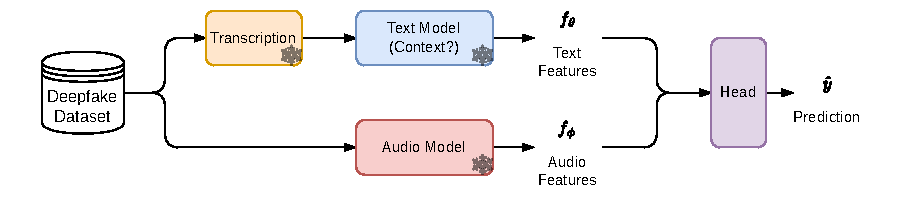
\includegraphics[width=1\textwidth]{figures/mid_fusion.pdf}
	\caption{Pipeline for Mid-Fusion}\label{fig:mid_fusion}
\end{figure*}


\begin{figure*}[t]
	\centering
	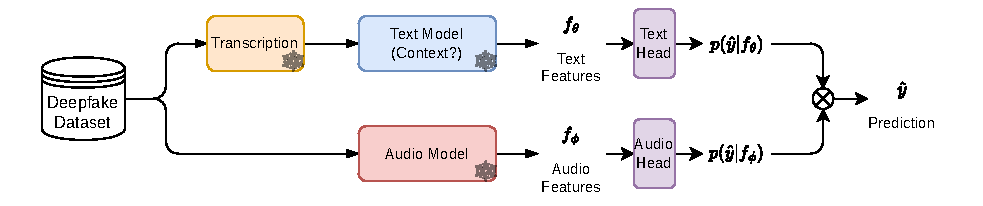
\includegraphics[width=1\textwidth]{figures/late_fusion.pdf}
	\caption{Pipeline for Late-Fusion}\label{fig:late_fusion}
\end{figure*}

\section{Experiments and Results}
\label{sec:experiments_results}

\section{Conclusions / Discussion}
\label{sec:conclusions}

\section{Acknowledgements}
Acknowledgement should only be included in the camera-ready version, not in the
version submitted for review. The 5th page is reserved exclusively for
acknowledgements and references. No other content must appear on the 5th page.
Appendices, if any, must be within the first 4 pages. The acknowledgments and
references may start on an earlier page, if there is space.

\ifinterspeechfinal
  The Interspeech 2025 organisers
\else
  The authors
\fi
would like to thank ISCA and the organising committees of past Interspeech conferences for their help and for kindly providing the previous version of this template.

\bibliographystyle{IEEEtran}
\bibliography{references}

\end{document}